\documentclass[tikz, border=1mm]{standalone}
\usepackage{tikz} 
\usetikzlibrary{arrows.meta}
\usepackage{pgfplots}

\pgfplotsset{compat=1.18}

\begin{document}

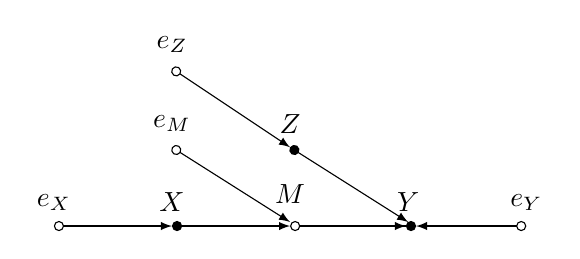
\begin{tikzpicture}

    % nodes (variables)
    \node at (-4.5,0) {$e_{X}$};
    \node at (-3,0) {$X$};
    \node at (-3,2) {$e_{Z}$};
    \node at (-1.5,1) {$Z$};
    \node at (-3,1) {$e_{M}$};
    \node at (-1.5,0.1) {$M$};
    \node at (0,0) {$Y$};
    \node at (1.5,0) {$e_{Y}$};
    
	% edges
    \draw[{Circle[open]}-{latex}](-4.5,-0.3) to (-3,-0.3); % e_{X} -> X
    \draw[{Circle[open]}-{latex}](-3,1.7) to (-1.5,0.7); % e_{Z} -> Z
    \draw[{Circle[open]}-{latex}](-3,0.7) to (-1.5,-0.25); % e_{M} -> M
    \draw[{Circle}-{latex}](-3,-0.3) to (-1.5,-0.3); % X -> M
    \draw[{Circle}-{latex}](-1.5,0.7) to (0,-0.25); % Z -> Y
    \draw[{Circle[open]}-{latex}{Circle}](-1.5,-0.3) to (0.1,-0.3); % M -> Y
    \draw[{Circle[open]}-{latex}](1.5,-0.3) to (0.1,-0.3); % e_{Y} -> Y    

\end{tikzpicture}

\end{document}
